\documentclass[10pt,a4paper]{article}
\linespread{1.2}
\usepackage{verbatim}
\usepackage{geometry}
\usepackage{listings}
\usepackage{graphicx}

\geometry{right=2.0cm,left=2.0cm,top = 2.0cm, bottom = 2.0cm}

\lstdefinestyle{mystyle}{
    basicstyle=\ttfamily
}

\lstset{style=mystyle}

\title{CAAM 419/519, Homework \#2}
\author{\texttt{hc54}}
\date{September 30, 2022}

\begin{document}

\maketitle

\section{Verification of the correctness of the two methods}


\begin{figure}[!ht]
        \centering 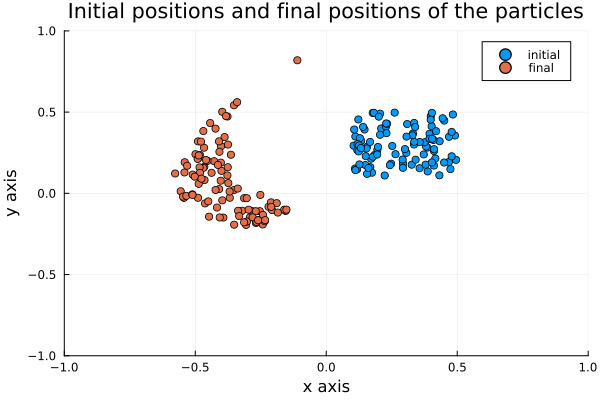
\includegraphics[scale=0.5]{figures/initialandfinal.png}
        \caption{Positions of the particles}
\end{figure}

\begin{figure}[!ht]
        \centering 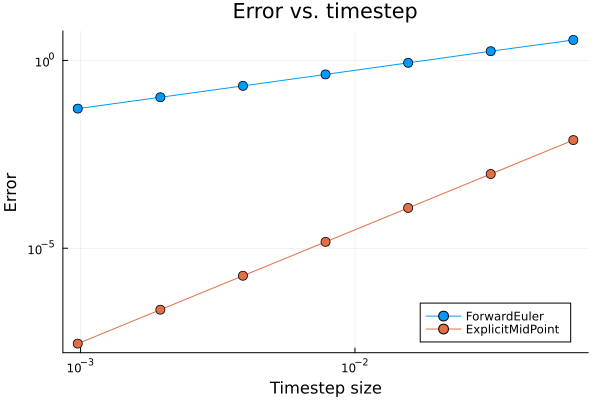
\includegraphics[scale=0.5]{figures/errorvsdt.png}
        \caption{Error vs dt}
\end{figure}

Explicit Midpoint Method performs better than Forward Euler Method. As timestep size decreases, the error of Explicit Midpoint Method decreases faster than Forward Euler Method and both error converges to 0. In addition, the error created by Explicit Midpoint Method is always less than the one created by Forward Euler among the seven tested timestep sizes. 


\section{Efficiency of rhs! function}

\begin{figure}[!ht]
        \centering 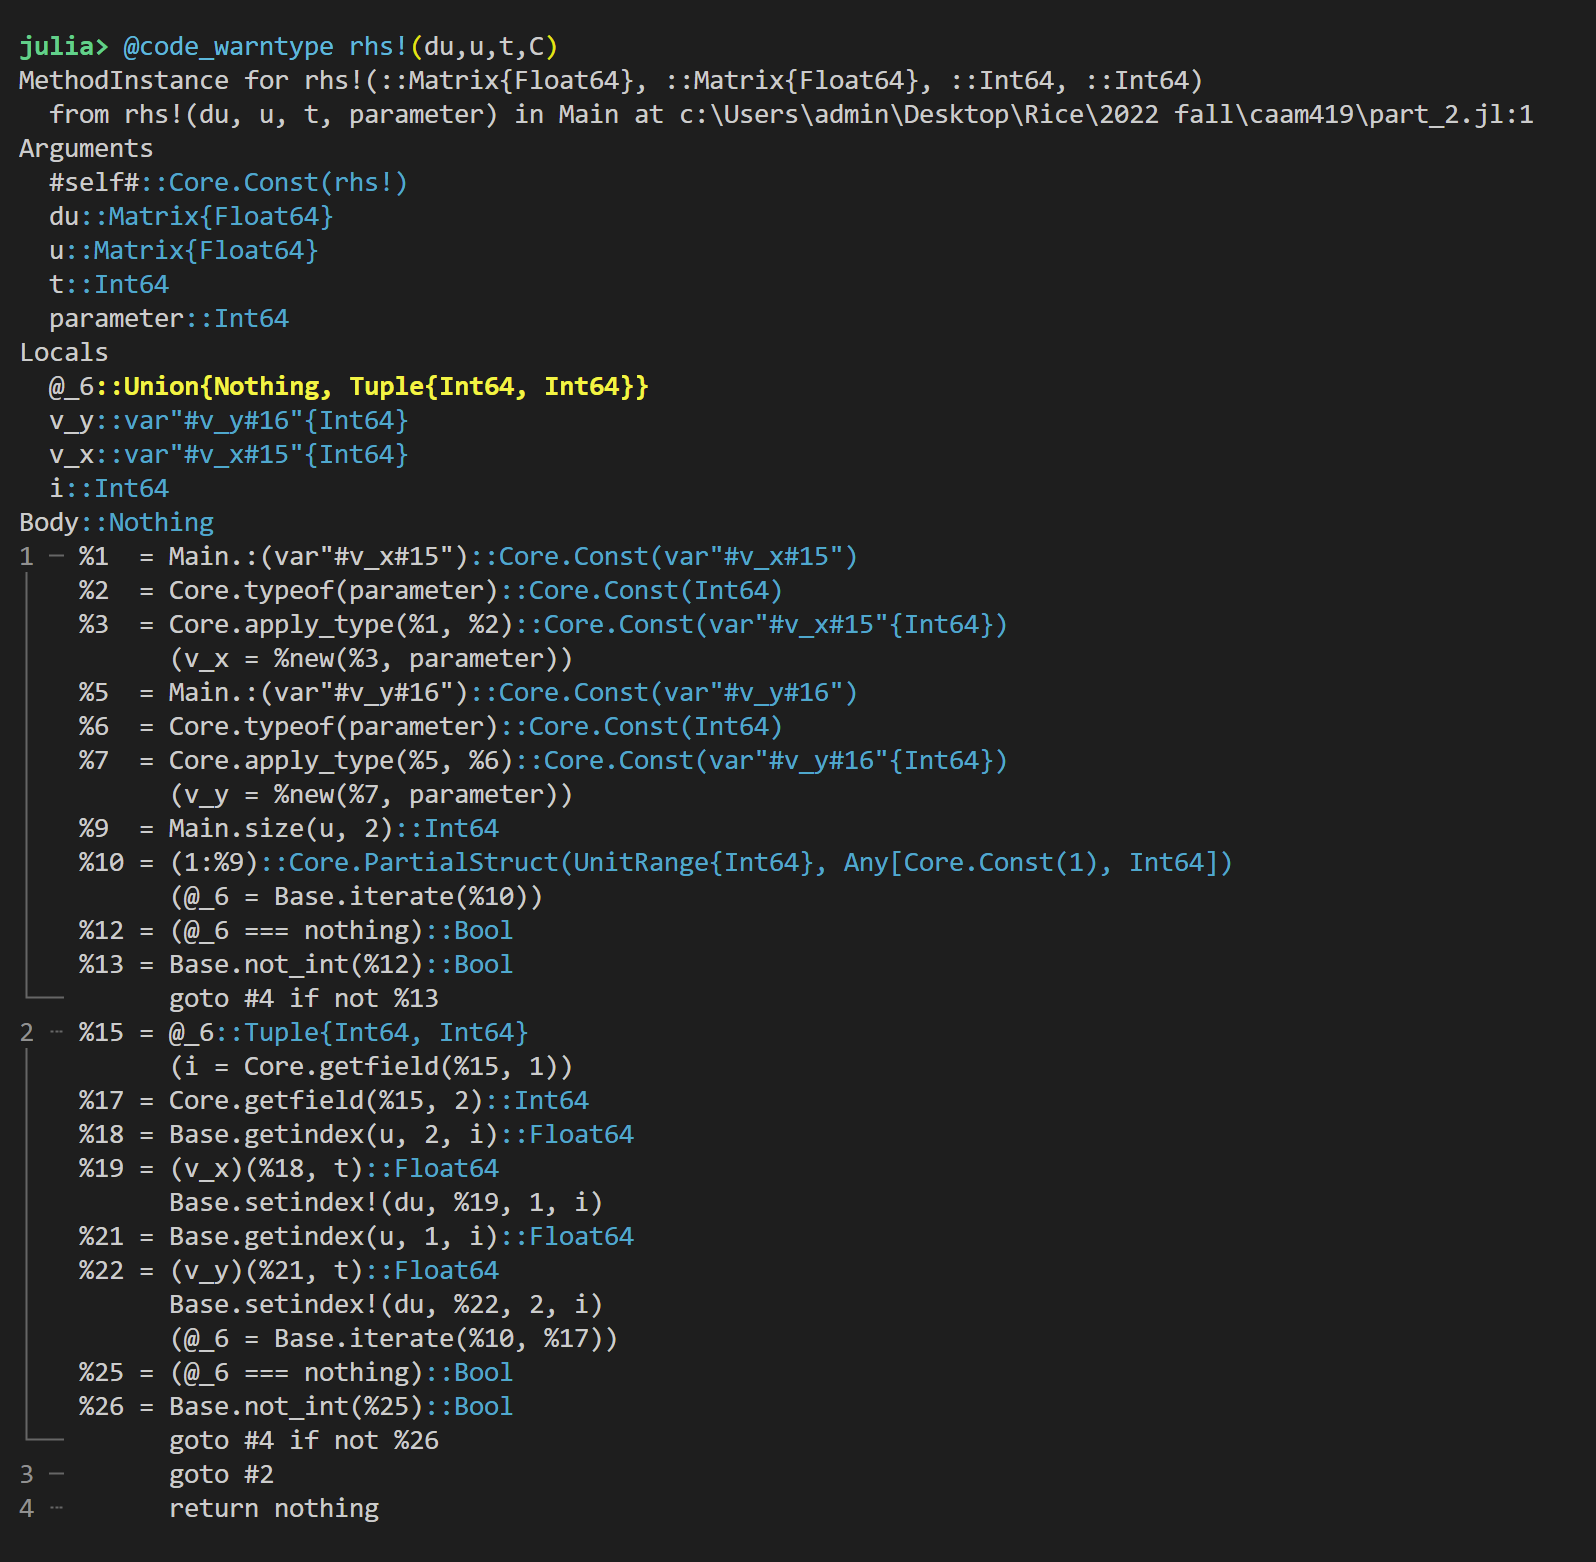
\includegraphics[scale=0.5]{figures/stability.png}
        \caption{Type stability}
\end{figure}

\noindent According to the output above, this function is type stable.

\begin{figure}[!ht]
        \centering 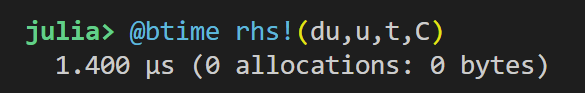
\includegraphics[scale=1]{figures/btime.png}
        \caption{Allocation}
\end{figure}

\noindent According to the output above, this function is allocation-free.

\section{Efficiency of solver function}

\begin{figure}[!ht]
        \centering 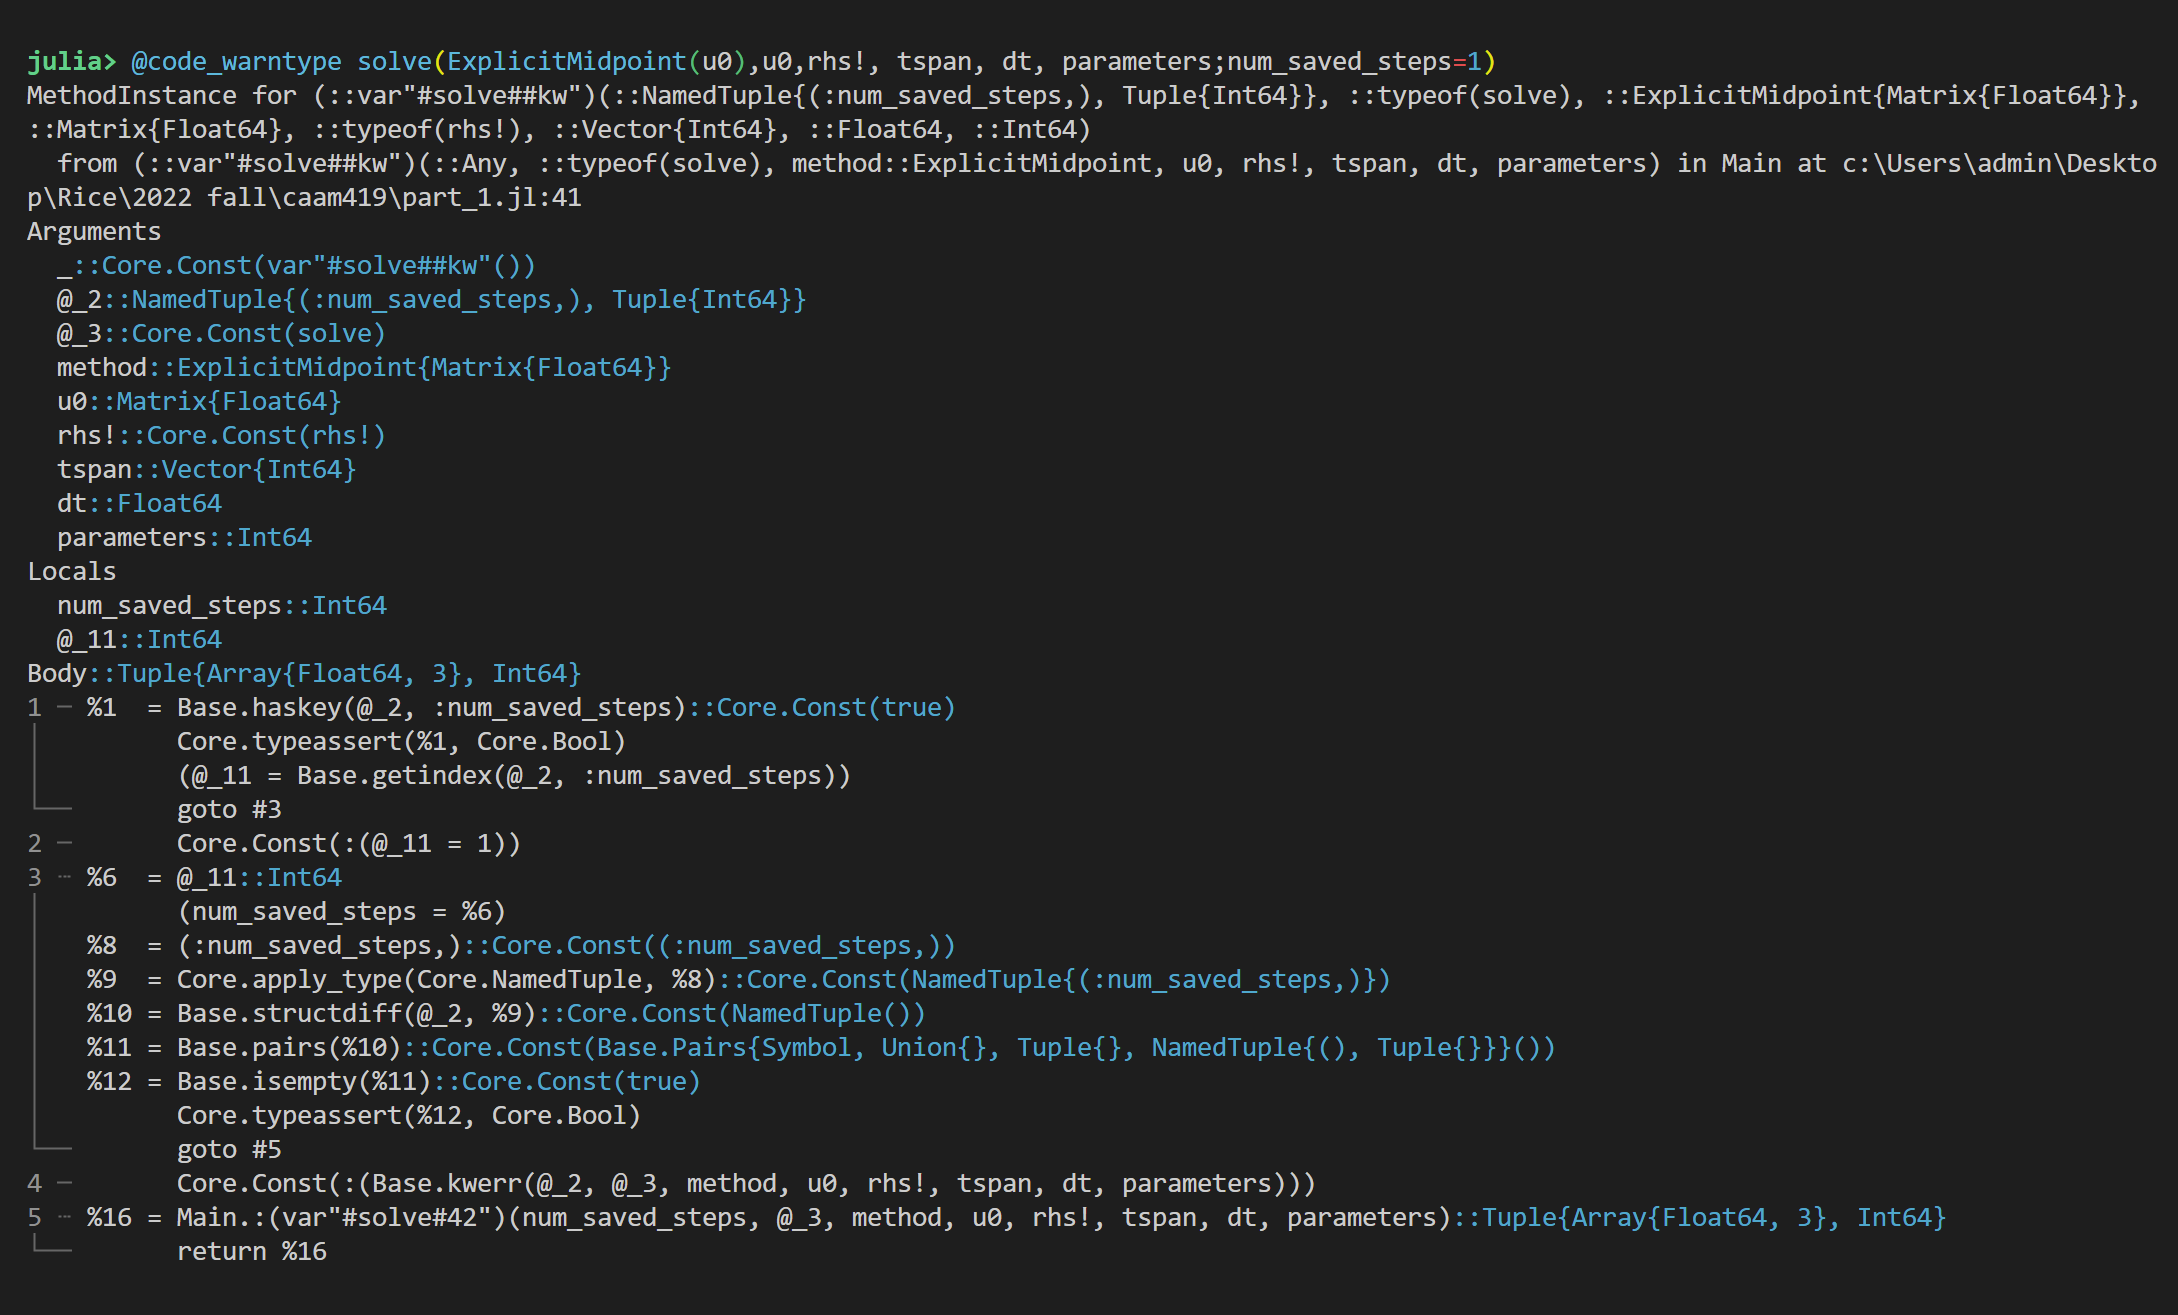
\includegraphics[scale=0.5]{figures/stability_solver1.png}
        \caption{Type stability for solver}
\end{figure}

\begin{figure}[!ht]
        \centering 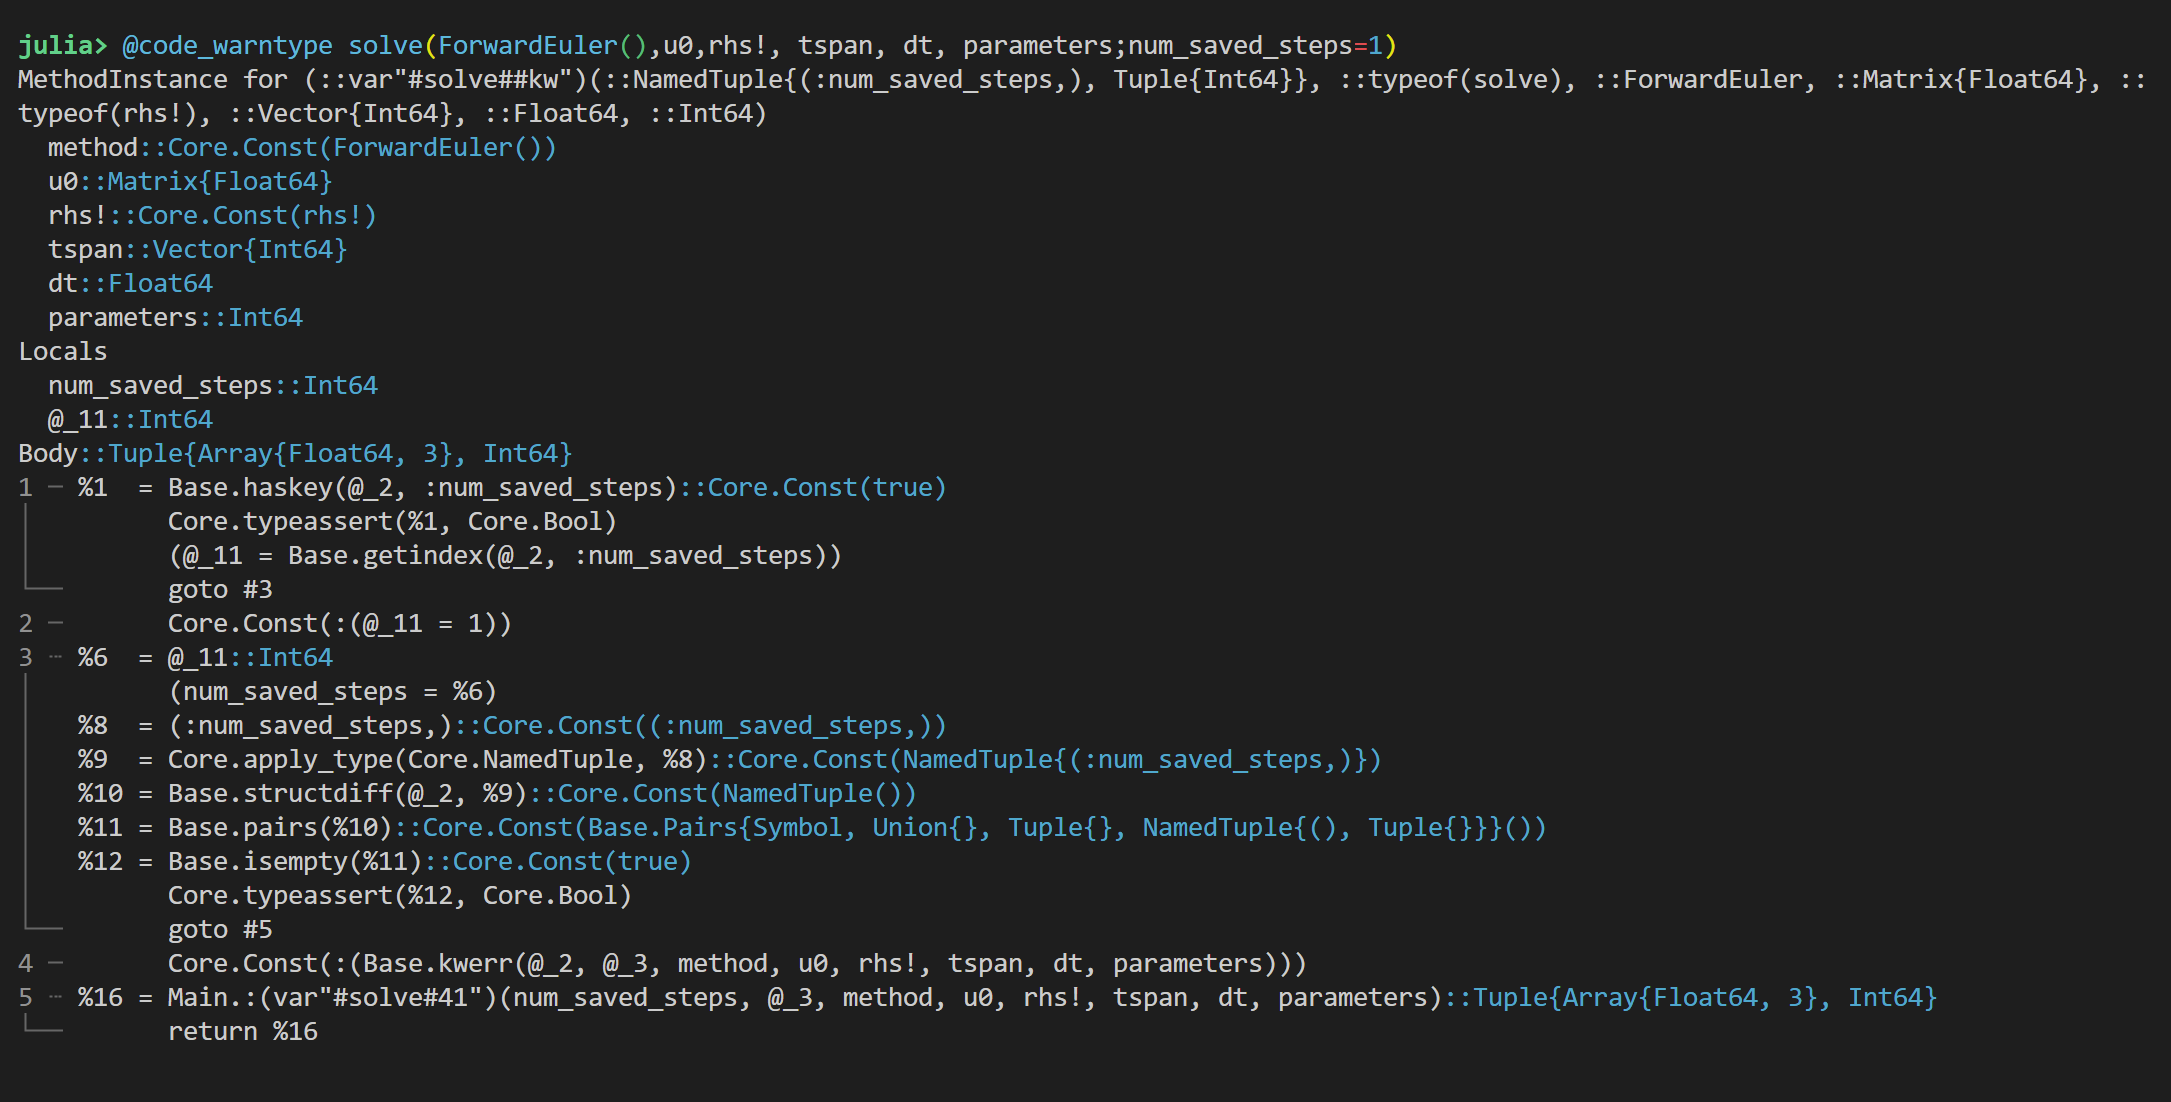
\includegraphics[scale=0.5]{figures/stability_solver2.png}
        \caption{Type stability for solver with another method}
\end{figure}

According to the outputs, the solver is type stable. 

\begin{figure}[!ht]
        \centering 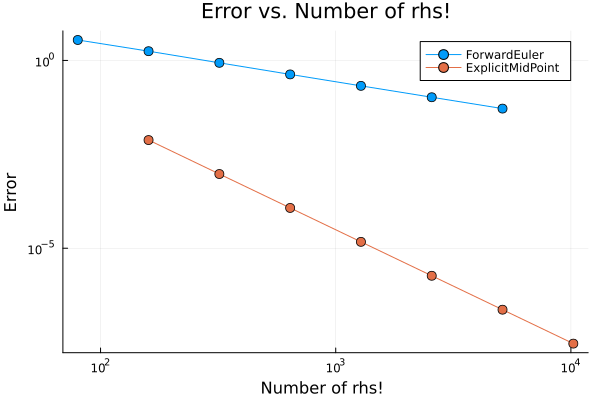
\includegraphics[scale=0.5]{figures/errorvsrhs.png}
        \caption{Error vs number of rhs! evaluations}
\end{figure}

\end{document}
